\documentclass[12pt]{report}
\usepackage{graphicx}
\usepackage{hyperref}

\title {
	
\includegraphics[width = .2\linewidth]{University-of-Lugano.png} \break \break
	{\bf\Huge Contextual Inquiry and Analysis}
	\\\large Human-Computer Interaction
	\\\small Academic Year 2017/2018 \break
	\\\large \textbf{Group 7}}
	\author{
	\\\large Alessandra Vicini \\ Edoardo Lunardi \\ Ozren Dabic \\ Pasquale Polverino \\ Paganoni Marco}
\date{March 02, 2018}
\begin{document}
	\pagestyle{empty}
	\maketitle
	\section*{\huge Our Research}
	We envisioned an application which could organize meetings
	between children based on their interests. We were aware of the fact 
	that our users were children and, keeping in
	this in mind, we tried to develop an idea, a concept with which
	children could be familiar with: and this was our main "topic" which led the
	interviews with children. The "field visit" let us understand properly
	what children expect from our application: during the interview we asked
	them about some of the features that we should include in the app. 
	We initially asked information regarding their interests, so that
	we would gather enough data to aid the development of our product. 
	We also faced the problem of the usage of smartphone: many children have some limitations for example,
	imposed by parents and also by the school which does not allow children
	to use their phone during certain time periods. Finally we revealed our idea to
	ensure that the application can be used only by children: we
	proposed that the access accounts may be given only by the school, and the
	children loved it. So in short, our "field visit" has
	asserted our ideas about the app and the children gave us some suggestions,
	which means a lot to us as far as future development is concerned.\\

	Upon reading the interviews from the remaining groups, we noticed 
	a similarity in the questions asked, although some were too vague, 
	and the information gathered from these questions was discarded, 
	since it would not be useful in the grand scheme of things. 
	Because of this, we tried to construct our flow model having the goal 
	of designing a sort of profile of all our users in order to satisfy all kinds of demands.\\

	By analysing all the interviews, we organized our work activity affinity diagram grouping the main points
	we have found into bigger subsets, 9 in total. Then we classified all the ideas
	from the interviews into each of the subsets. The most difficult part was finding groups under
	which structered our work. Our subsets were mainly based on the children
	answers and also we have looked for face the topics argued in class, for
	example the privacy and the safety of the applications, problems whose we
	have also a solution in our app and also children knows it. In the end our diagram
	is composed by three main concepts: what children expects and want from the app,
	how we can deal with this in creating something which attracts them and also ethical
	problems, which must be taken in consideration just because we are talking about
	children. Our work looked this way: \\\\\\
	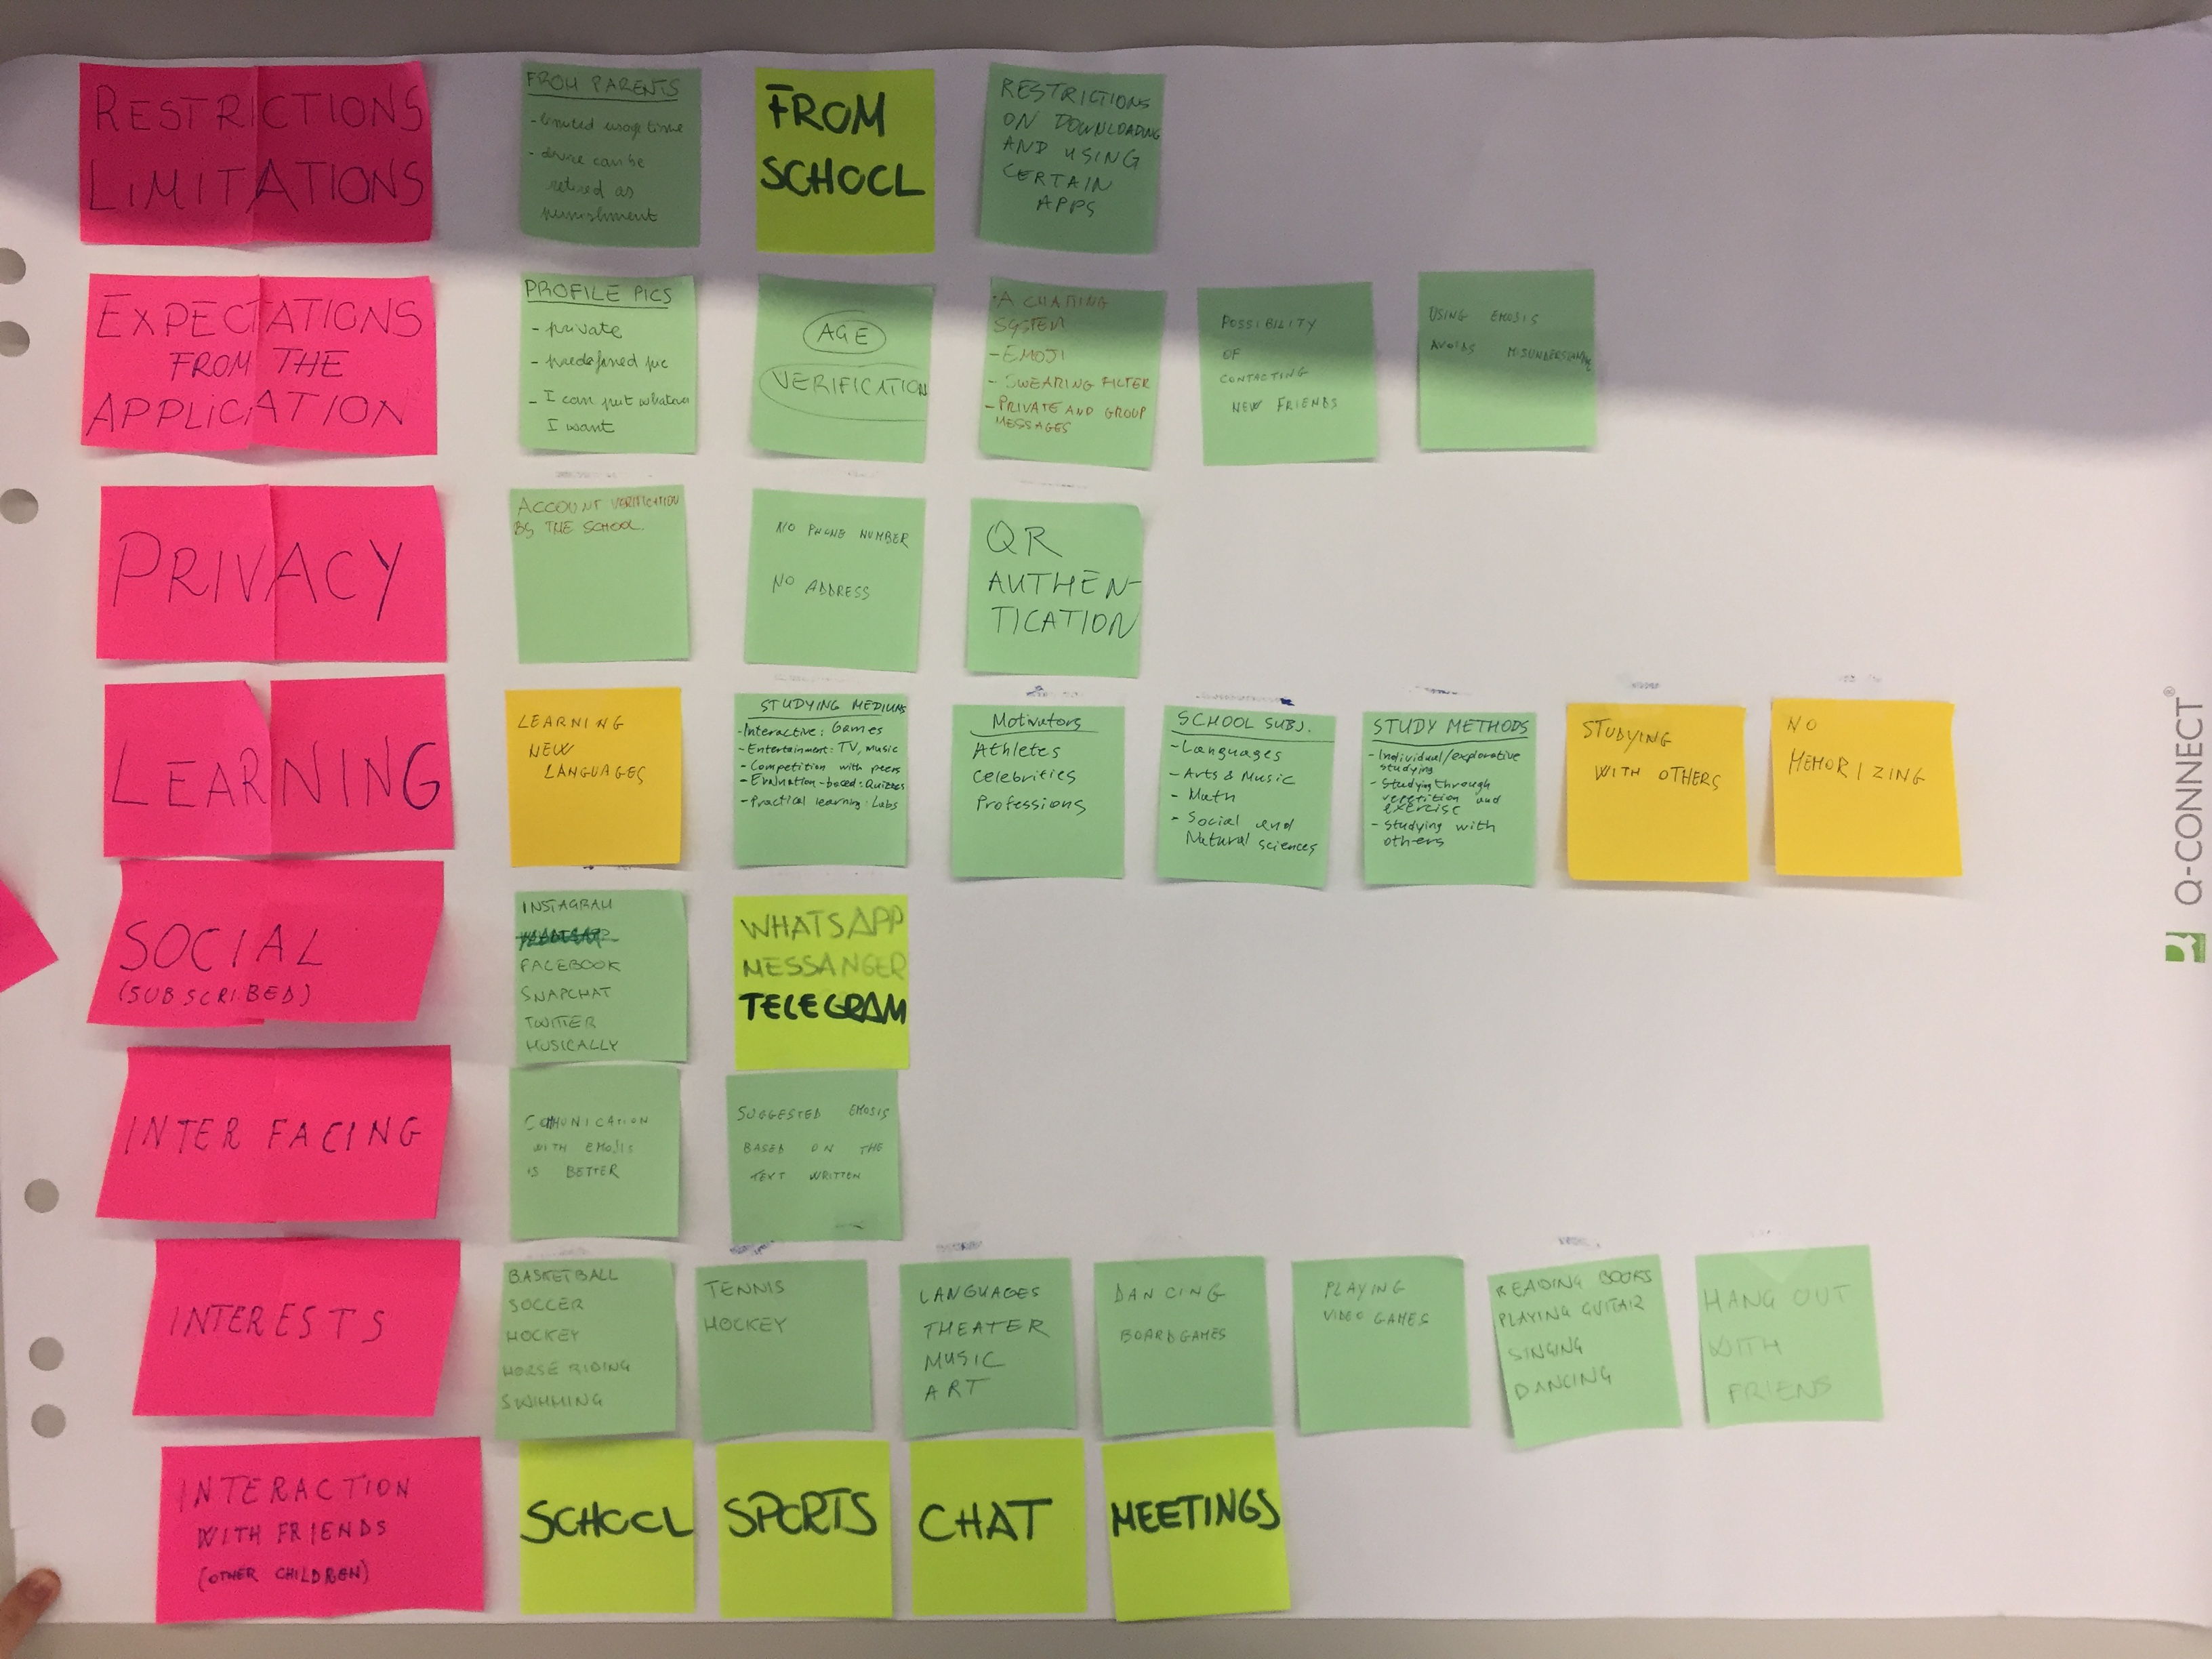
\includegraphics[width = 1.0\linewidth]{affinity_diagram.jpg}\break

  As clearly visible in the diagram we create 9 subsets and each of them has its
  main topics, designed reading the interviews. These are our groups:
	\begin{itemize}
		\item "Restrictions and Limitations":\\
		       we created this subset because we noticed that most children have
					 restrictions and limitations regarding the usage of their phones.
		\item "Expectations from the application" :\\
		       this was an obvious topic to take into consideration, the application is designed
					 for children and they have to be the users: it is our duty to listen to their requests and expectations. 
					 We also noticed that some of their expectations matched our initial product idea.
		\item "Privacy":\\
		       that is the main ethical problem, and just because our users will be children,
					 we will put more attention on this part and also on how to make the app safer and more reliable.
		\item "Learning":\\
		       some children expect an application which will help them to learn new things, so even if this wasn't
					 part of our original idea we could think of implementing something akin to that.
		\item "Social":\\
		       this point focus on the design of the most famous social app: if children are more familiar
					 with a certain type of design, we will try to create something as similar as possible.
		\item "Interfacing":\\
		       many children suggested the usage of emojis in communication. Our app will include a sort
					 of live chat, so this is a great suggestion for us.
		\item "Interests":\\
		       this is the meat of our application, so we listed the most common interests and hobbies
					 so that we can include them in our product.
		\item "Interaction with friends:"\\
		       we make sure that children are used to go out with friends and they have the possibility to do
					 it and if not why not and try to solve the problem.

	\end{itemize}

	 This was our analysis of the project in the entire context, keeping in mind who are our users and what we
	 plan to do considering them. Each part of the project has been structured having in mind children, what we
	 know has been learned by the interview and also analyzing the draws of children. Our group worked toghether
	 to reach the best result possible, we are all satisfied.














	\end {document}
